% ============================================================================
% M4 contribution split by IMRaD part (Introduction, Methods, Results,
% Discussion) plus an Appendix block, PNAS template (pnas-new.cls) with
% Methods BEFORE Results, as requested by the instructor. The paper body shows
% only the main estimate (matched + not-yet-treated controls); alternative
% control groups, the TWFE comparison, other outcomes and robustness checks are
% in the Appendix block, and their main implications are summarised in the
% Results block. Block 6 is a "further analysis" appendix for the
% affordability part (alternative tax-deduction scenarios for net income).
%
% Each block below goes INSIDE the group's corresponding section, after the
% parts written by the other members. The blocks do not open their own
% \section: they use \subsection* (Methods, Results) or plain paragraphs
% (Introduction, Discussion), so they continue the text around them.
%
% Before pasting, check the phrases marked [LINK]: they refer to the other
% parts of the paper (affordability index, data section) and may need to be
% adapted to the final wording of those parts.
%
% Files: upload m4_cs_event_rent_en.png to Overleaf; add m4_refs.bib entries
% to the project bibliography.
% ============================================================================


% ############################################################################
% 1. INTRODUCTION  --  paste after the paragraphs that motivate the paper and
%    present the affordability question (two paragraphs, no heading)
% ############################################################################

A natural question is whether new transit infrastructure contributes to these rent dynamics. % [LINK] "these" = the rent increases presented in the paragraphs before
The capitalisation of accessibility predicts that better transit access lowers commuting costs and raises the price of housing close to new stations \cite{alonso1964,gibbons2005}; empirical studies of new rail lines generally find positive but modest and very local effects \cite{billings2011}, and in Italy Daniele and Romito \cite{daniele2022} use OMI zone quotations, the data source we also rely on, to study the opening of Metro C in Rome. Milan's M4 line, opened in three stages between November 2022 and October 2024, offers a staggered natural experiment in the middle of the period we study.

We therefore also ask whether the M4 changed residential rents in the zones it served for the first time. Using a heterogeneity-robust difference-in-differences design \cite{callaway2021} with permutation inference, we find no robust evidence that the line raised OMI rent quotations in the five newly served zones over the first three to seven semesters after opening.


% ############################################################################
% 2. METHODS  --  paste after the description of the data and of the
%    affordability index
% ############################################################################

\subsection*{Effect of the M4 Line on Local Rents}

\paragraph{Data.} We use the OMI rent quotations described above at the level of OMI zones rather than neighbourhoods. % [LINK] refers to the data subsection on OMI quotations
For each zone and semester we take the midpoint of the range for residential units in normal condition, in euros per square metre of gross floor area per month. The panel runs from 2014S2 to 2026S1, the period with a consistent zoning map; we keep the zones with a rent quotation in every semester (a balanced panel of 37 zones) and take 2026S1, not yet in the municipal release, directly from the Agenzia delle Entrate. Values are nominal: deflating by a price index common to all zones would leave every estimate unchanged, because the common term cancels in the double difference (we verified this numerically). Station coordinates and line membership come from the municipal open-data portal (dataset ds535).

\paragraph{Treatment definition and timing.} An area is treated when at least 20\% of its surface gains new metro access within 500 metres of an M4 station. We overlay a regular grid of points on the city; a point is \textit{newly served} if it lies within 500~m of an M4 station and more than 500~m from any station of the other lines (M1, M2, M3, M5). An area's exposure to a section is the share of its grid points newly served by that section's stations. An area is treated if its exposure reaches 20\%, and \textit{never exposed} if no point lies within 500~m of any M4 station; partially exposed areas, and areas near the M4 already served by other lines, are excluded. The 500~m radius matches the walking catchment of an urban station and is close to the median distance between consecutive M4 stations (469~m). The first treated period is the first semester during which the section was open for all or almost all of the period (Table~\ref{tab:m4timing}). Section 2 serves no zone for the first time, because Tricolore and San Babila are within 500~m of the M1 and M3 lines; five OMI zones are therefore treated, one from 2023S1 and four from 2025S1.

\begin{table*}[tbhp]
\centering
\caption{M4 opening dates and treated OMI zones (500~m catchment, 20\% exposure threshold)}
\label{tab:m4timing}
\resizebox{\textwidth}{!}{%
\begin{tabular}{llcccl}
\hline
Section & Opening & Opening semester & First treated & Post-opening semesters & Treated zones \\
 & & (share of days open) & semester & to 2026S1 & \\
\hline
1 Linate--Dateo & 26 Nov 2022 & 2022S2 (20\%) & 2023S1 & 7 & 1 (D12) \\
2 Dateo--San Babila & 4 Jul 2023 & 2023S2 (98\%) & 2023S2 & 6 & 0 \\
3 San Babila--San Cristoforo & 12 Oct 2024 & 2024S2 (44\%) & 2025S1 & 3 & 4 (B13, B20, B21, D24) \\
\hline
\end{tabular}}
\addtabletext{Source: authors' elaboration on OMI and municipal open data.}
\end{table*}

\paragraph{Target parameter and identification.} The estimand is the average effect of gaining new M4 access on the log OMI midpoint rent of the five treated zones, over the semesters observed after their opening, relative to the counterfactual path given by the controls. Identification requires (\textit{i}) parallel trends: absent the line, treated zones and their controls would have followed the same rent path from the reference semester onwards; (\textit{ii}) no anticipation between the reference semester and opening; and (\textit{iii}) no spillovers of the line onto the control zones. The estimate is therefore a relative effect, which differences out any effect of the line common to the whole city; it concerns OMI quotations, which are appraisal-based ranges rather than transaction rents; and it says nothing about effects beyond the observed three to seven semesters.

\paragraph{Estimator.} Because the sections opened at different dates, a two-way fixed-effects regression would use already-treated zones as controls for later-treated ones, which can bias the estimate when effects vary over time \cite{goodmanbacon2021,dechaisemartin2020}. We instead use the estimator of Callaway and Sant'Anna \cite{callaway2021}. Let $g$ be the first treated period of a group and $b=g-1$ a common reference period. For log rent $Y$,
\begin{equation}
\mathrm{ATT}(g,t)=\left[\bar Y_{g,t}-\bar Y_{g,b}\right]-\left[\bar Y_{C(g,t),t}-\bar Y_{C(g,t),b}\right],
\label{eq:attgt}
\end{equation}
where the control set $C(g,t)$ contains the sample zones that are never exposed or that open after $\max(t,b)$, and means are unweighted across zones. The headline estimate averages the post-opening effects, weighting each group by its number of treated zones $n_g$:
\begin{equation}
\mathrm{ATT}=\frac{\sum_g\sum_{t\ge g} n_g\,\mathrm{ATT}(g,t)}{\sum_g\sum_{t\ge g} n_g},
\label{eq:attagg}
\end{equation}
so that section 1 (one zone $\times$ 7 semesters) receives weight 7/19 and section 3 (four zones $\times$ 3 semesters) 12/19. Aggregating by time relative to opening, $e=t-g$, gives the event study
\begin{equation}
\mathrm{ES}(e)=\frac{\sum_g n_g\,\mathrm{ATT}(g,g+e)}{\sum_g n_g},
\label{eq:es}
\end{equation}
with the sums over the groups observed at $e$ and $\mathrm{ES}(-1)=0$ by construction. The average pre-opening coefficient over $e=-8,\dots,-2$ is reported as a placebo.

\paragraph{Control group.} For each treated zone we select the three never-exposed zones most similar before the metro, by Euclidean distance on standardised covariates (2014--2016 levels of log rents and log prices, 2014--2019 growth of log rents, and the 2014 shares of foreign residents, residents aged 65 and over, and single-person households, mapped from neighbourhoods to zones by area overlap). This yields six matched controls, to which zones of later sections are added as not-yet-treated controls until they open. The Appendix reports two alternative control groups (all 20 never-exposed zones, and not-yet-treated zones only).

\paragraph{Inference.} With five treated zones, cluster-robust standard errors are unreliable \cite{conley2011,mackinnon2018}, so we base inference on randomisation. We test the sharp null that the M4 had no effect on any zone in any semester: in the main sample of 11 zones we randomly reassign the opening-group labels (one zone opening in 2023S1, four in 2025S1, six controls), keeping the number of zones per group fixed, and recompute the full estimator for each of 999 draws (out of 2,310 distinct assignments). The two-sided $p$-value is $p=(1+\#\{|\mathrm{ATT}_p|\ge|\mathrm{ATT}|\})/(1+B)$. It has exact finite-sample level only if, under the null, the observed assignment of opening dates is one equally likely draw among the relabellings; since the dates were set by the route of the line and the treated zones are central, this exchangeability is a maintained assumption, and the test conditions on the matched sample, which is not re-drawn within permutations. For the main estimate and the alternative control groups we obtain 95\% confidence intervals by inverting the permutation test under a constant additive effect \cite{imbens2015}: a value $\delta$ is in the interval if the test of no effect applied to $Y-\delta D$, with $D=1$ for treated zones after their own opening, does not reject at 5\%. For robustness checks and event-study coefficients we use the faster approximation estimate $\pm c$, where $c$ is the 95th percentile of the permuted $|$estimates$|$, and a simultaneous sup-$t$ band \cite{montielolea2019} built from the same permutation distribution over $e=-12,\dots,6$ ($\hat c=2.40$). Under the same constant-effect approximation, the minimum detectable effect with 80\% power, the smallest $\delta$ such that $P(|\delta+e|\ge c)\ge0.8$ for permuted estimates $e$, is 9.4\%.


% ############################################################################
% 3. RESULTS  --  paste after the results of the affordability analysis
% ############################################################################

\subsection*{Effect of the M4 Line on Local Rents}

Rents did not increase in the newly served zones after the M4 opened. Over the semesters observed after opening, rents in the five newly served zones grew 4.6\% less than in their matched controls (permutation $p=0.13$, 999 relabellings of the opening groups). Under the constant-effect assumption, effects outside $[-9.7\%,+2.2\%]$ are rejected at the 5\% level, so rent increases larger than about 2\% are inconsistent with the data, while decreases of up to about 10\% cannot be ruled out. The average pre-opening coefficient over $e=-8,\dots,-2$ is $+0.028$ log points ($p=0.52$).

\begin{figure*}[tbhp]
\centering
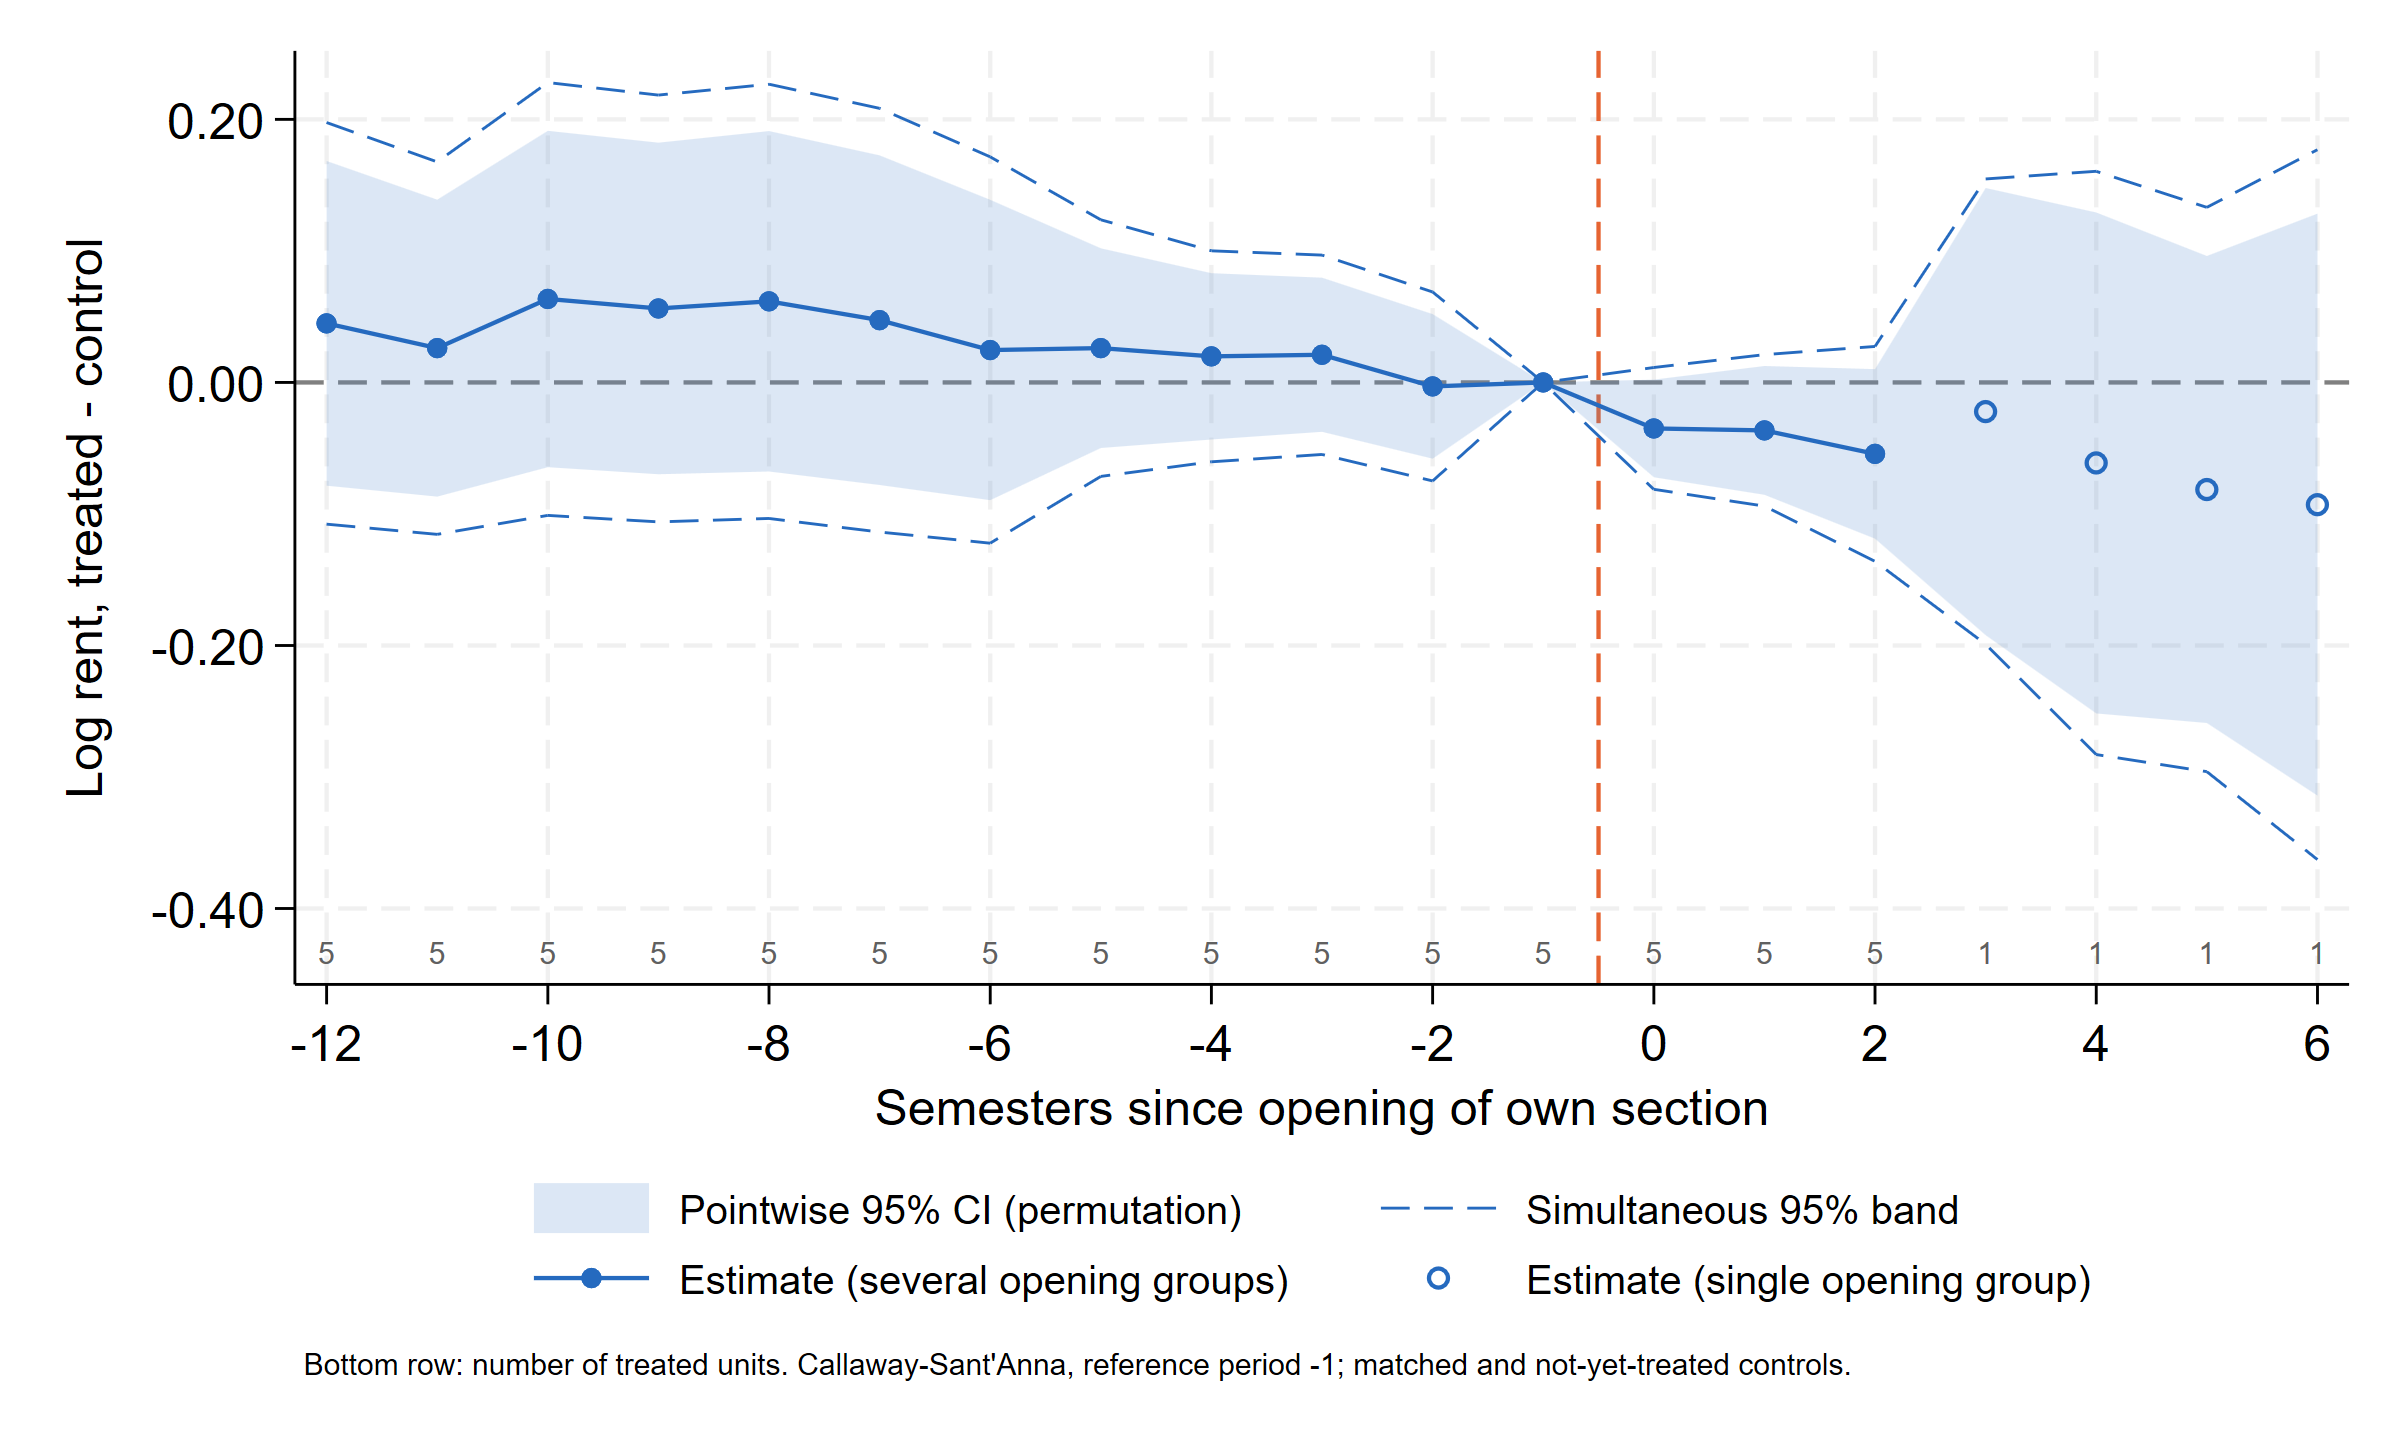
\includegraphics[width=0.8\textwidth]{m4_cs_event_rent_en.png}
\caption{Event study: log rent, zones newly served by the M4 vs.\ matched and not-yet-treated controls. Callaway--Sant'Anna coefficients by semester relative to opening (reference $e=-1$). Shaded area: approximate pointwise 95\% intervals; dashed lines: approximate 95\% simultaneous sup-$t$ band over $e=-12,\dots,6$, both from 999 permutations of the opening groups. Bottom row: number of treated zones in each coefficient; hollow markers rest on a single opening group.}
\label{fig:m4event}
\end{figure*}

Figure~\ref{fig:m4event} shows the event study. Before opening, rents in M4 zones were 4 to 6 log points above matched controls up to $e=-7$ and converged steadily to zero by $e=-1$. No pre-opening coefficient is individually significant and the simultaneous band contains zero for all of them, but the point estimates trace a gradual relative decline that started years before the line opened, and the pre-test has little power with five treated zones. After opening, the first three coefficients are $-0.035$ (95\% CI $-0.072$ to $+0.002$), $-0.036$ and $-0.054$. From $e=+3$ to $+6$ the coefficients rest on a single zone (D12), so the further fall to $-0.09$ reflects the change in composition rather than a growing effect.

The alternative specifications and robustness checks reported in the Appendix (Tables~\ref{tab:m4controls}--\ref{tab:m4sdid}) have four main implications. First, the result does not depend on the matching: with all 20 never-exposed zones as controls the estimate is $-4.0\%$ ($p=0.24$), while using only zones that open later gives an uninformative $+3.2\%$ (approximate CI $-4.6\%$ to $+11.7\%$), based on one treated zone over four semesters. Second, it does not depend on the exact treatment definition: with catchments of 800 or 1,000~m and exposure thresholds of 10\% or 30\%, the estimate stays between $-1\%$ and $-6\%$, and it becomes significant only with the 10\% threshold, which doubles the number of treated zones ($-4.6\%$, $p=0.036$). Third, it is not driven by a single zone or by the timing of treatment: leaving out one treated zone at a time gives estimates between $-3.6\%$ and $-5.6\%$, and excluding the partly served reference semesters leaves it unchanged ($-4.4\%$). Fourth, a synthetic difference-in-differences estimator \cite{arkhangelsky2021}, which reweights controls and pre-opening periods to match the pre-opening path of the treated zones, gives $-3.8\%$ (95\% CI $-10.2\%$ to $+3.0\%$), close to the main estimate; the much larger $-12.2\%$ of a two-way fixed-effects regression comes from its reference period rather than from the staggered timing. No check points to a rent increase in the newly served zones.


% ############################################################################
% 4. DISCUSSION  --  paste after the discussion of the affordability results
% ############################################################################

The M4 analysis complements these findings. % [LINK] "these findings" = the affordability results discussed just before
In the five newly served OMI zones and over the first three to seven semesters after opening, we find no robust evidence of an increase in rent quotations, relative to comparable zones, attributable to the new line. Under the maintained assumptions, relative increases larger than about 2\% are inconsistent with the data, but the estimates cannot distinguish a zero effect from a moderate decrease. The negative point estimates should not be read as a causal fall in rents either: the relative decline of the served zones began before the line opened, and the design cannot separate a possible effect of the line from that trend. For the affordability question, the 2022--2024 rise in rents documented above does not appear concentrated in the zones newly served by the M4; because the design identifies a relative effect, however, it cannot speak to effects of the line common to the whole city.

Several features of the setting limit these conclusions. Only five zones are treated, so power reaches 80\% only for effects of about $\pm9\%$, and the permutation $p$-value has exact level only if opening dates are exchangeable across the sample zones, which the route of the line does not guarantee. Newly served zones are mostly central while clean controls are more peripheral, so a divergence between centre and periphery over the same years is confounded with the effect of the line; the positive pre-opening placebo points in this direction. The line was announced and construction began before 2014, so any capitalisation at announcement predates our panel, and OMI zones are much larger than a station's catchment, which dilutes a local effect. Longer post-periods and finer spatial data, such as station-level listings, would allow a sharper test.


% ############################################################################
% 5. APPENDIX  --  paste in the group's appendix (after the references, or in
%    the appendix section the group uses). If the group appendix already
%    restarts table numbering, drop the two \renewcommand/\setcounter lines.
% ############################################################################

\subsection*{Appendix: Alternative Specifications and Robustness of the M4 Estimates}
\renewcommand{\thetable}{A\arabic{table}}
\setcounter{table}{0}

This appendix reports the alternative specifications and robustness checks summarised in the Results. All estimates use the log OMI midpoint rent, the Callaway--Sant'Anna estimator with matched and not-yet-treated controls and permutation inference, unless stated.

\paragraph{Alternative control groups.} Table~\ref{tab:m4controls} compares the main estimate with two specifications that differ only in the control group. (2) \textit{All never-exposed + not-yet-treated} uses all 20 never-exposed zones instead of the six matched ones, to test whether the result depends on the matching; the estimate is very similar ($-4.0\%$). (3) \textit{Not-yet-treated only} uses only zones of sections that open later, which were selected by the same planning process; once the last section opens no control is left, so this specification compares the single section-1 zone with the four section-3 zones up to 2024S2. Its estimate is positive but very imprecise, and we treat it as uninformative.

\begin{table*}[tbhp]
\centering
\caption{Effect of the M4 opening on log rents: alternative control groups (Callaway--Sant'Anna)}
\label{tab:m4controls}
\resizebox{\textwidth}{!}{%
\begin{tabular}{llcccccc}
\hline
 & Controls & ATT & 95\% CI & Permutation & Pre-opening & Treated / never- & Period \\
 & & & & $p$ & placebo ($p$) & exposed controls & \\
\hline
(1) Main & Matched + not-yet-treated & $-4.6\%$ & $[-9.7\%, +2.2\%]$ & 0.133 & $+0.028$ (0.52) & 5 / 6 & 2014S2--2026S1 \\
(2) & All never-exposed + not-yet-treated & $-4.0\%$ & $[-9.6\%, +2.4\%]$ & 0.243 & $+0.052$ (0.20) & 5 / 20 & 2014S2--2026S1 \\
(3) & Not-yet-treated only & $+3.2\%$ & $[-4.6\%, +11.7\%]^{a}$ & 0.625 & $-0.045$ (0.62) & 5 / 0 & 2014S2--2024S2 \\
\hline
\end{tabular}}
\addtabletext{Outcome: log of the OMI midpoint rent; OMI zones, semesters. Percentages are $100\times(\exp(\mathrm{ATT})-1)$. Permutation $p$-values use 999 random relabellings of the opening groups. 95\% intervals invert the permutation test under a constant additive effect; $^{a}$approximate interval (estimate $\pm c$). The placebo is the average pre-opening coefficient over $e=-8,\dots,-2$, in log points.}
\end{table*}

\paragraph{Two-way fixed effects.} A two-way fixed-effects regression of log rent on a treatment indicator with zone and semester fixed effects and standard errors clustered by zone gives $-12.2\%$. The gap with the main estimate does not come from the staggered timing: a plain difference-in-differences, which makes no comparison between already-treated and later-treated zones, gives a similar value ($-12.5\%$, Table~\ref{tab:m4sdid}). It comes from the reference period, which for these regressions is the average of all pre-opening semesters, during which the served zones were declining relative to the controls, whereas the main estimator compares each post-opening semester with the semester before opening.

\paragraph{Other outcomes.} With the same design we also examined OMI sale prices (OMI zones, semesters) and resident out-migration (neighbourhoods, years; three treated neighbourhoods observed after the first opening, 2023--2024). Neither shows a robust effect: prices $-3.1\%$ ($p=0.27$); out-migration $-2.4$ per 1,000 residents ($p=0.07$), falling to $-1.0$ ($p=0.51$) with an earlier reference year.

\paragraph{Treatment definition.} We change the catchment radius (800 and 1,000~m instead of 500~m) and the exposure threshold (10\% and 30\% instead of 20\%), keeping everything else fixed. The estimate is similar with an 800~m catchment or a 10\% or 30\% threshold and smaller with a 1,000~m catchment. With the 10\% threshold the number of treated zones doubles to ten and the estimate becomes significant ($-4.6\%$, $p=0.036$), with the same sign and size as the main estimate.

\paragraph{Influential zones.} Dropping one treated zone at a time keeps the estimate between $-3.6\%$ and $-5.6\%$, with $p$-values between 0.05 and 0.23.

\paragraph{Classification of opening periods.} The reference semester is partly treated for two sections: 2022S2 was served for 20\% of its days (section 1) and 2024S2 for 44\% (section 3). Using $g-2$ as reference, so that the partially treated semester enters neither the base nor the effects, gives $-4.4\%$; dating treatment from the opening semester itself gives $-3.5\%$.

\paragraph{Synthetic difference-in-differences.} The estimator of Arkhangelsky et al.\ \cite{arkhangelsky2021} chooses weights for the control zones and for the pre-opening semesters so that the weighted controls track the treated zones before opening. On the same balanced sample and horizon (5 treated, 20 never-exposed zones), Table~\ref{tab:m4sdid} compares it with Callaway--Sant'Anna and with a plain difference-in-differences. The pre-trend is the mean of $[(\text{treated}-\text{control})_t-(\text{treated}-\text{control})_{g-1}]$ over $e=-8,\dots,-2$, measured in the same way for all methods. The plain difference-in-differences, which uses the average of all pre-opening semesters as reference, is much more negative; once controls and periods are reweighted, the pre-trend falls from 0.054 to 0.015 log points and the estimate is close to Callaway--Sant'Anna and insignificant. Unit weights spread over about 11 effective controls, with a maximum weight of 0.17; time weights concentrate on the semester before opening (66\% for section 1, 97\% for section 3).

\begin{table}[tbhp]
\centering
\caption{Robustness checks, log rent}
\label{tab:m4robust}
\begin{tabular}{lccc}
\hline
Check & Estimate & $p$ & Treated \\
\hline
Main specification (1) & $-4.6\%$ & 0.13 & 5 \\
Catchment 800 m & $-5.2\%$ & 0.42 & 3 \\
Catchment 1,000 m & $-1.3\%$ & 0.80 & 4 \\
Exposure threshold 10\% & $-4.6\%$ & 0.036 & 10 \\
Exposure threshold 30\% & $-4.2\%$ & 0.32 & 2 \\
Leave one treated zone out & $-3.6$ to $-5.6\%$ & 0.05--0.23 & 4 \\
Reference period $g-2$ & $-4.4\%$ & 0.40 & 5 \\
Treatment from opening semester & $-3.5\%$ & 0.45 & 5 \\
Synthetic DiD & $-3.8\%$ & 0.27 & 5 \\
\hline
\end{tabular}
\addtabletext{Callaway--Sant'Anna with matched and not-yet-treated controls and permutation $p$-values, unless stated. Catchment and threshold variants use 499 permutations. The synthetic DiD uses all never-exposed zones; its $p$-value comes from placebo standard errors and a normal approximation, not from the permutation test.}
\end{table}

\begin{table}[tbhp]
\centering
\caption{Same sample and horizon: Callaway--Sant'Anna, difference-in-differences and synthetic DiD}
\label{tab:m4sdid}
\resizebox{\columnwidth}{!}{%
\begin{tabular}{lcccc}
\hline
Method & Estimate & 95\% CI & $p$ & Pre-trend \\
\hline
C\&S, never-exposed controls & $-4.1\%$ & $[-10.4\%, +2.7\%]$ & 0.23 & $+0.054$ \\
Difference-in-differences & $-12.5\%$ & $[-21.6\%, -2.4\%]$ & 0.017 & $+0.054$ \\
Synthetic DiD & $-3.8\%$ & $[-10.2\%, +3.0\%]$ & 0.27 & $+0.015$ \\
\hline
\end{tabular}}
\addtabletext{5 treated and 20 never-exposed zones, 2014S2--2026S1. C\&S: permutation $p$ and approximate interval (estimate $\pm c$); difference-in-differences and synthetic DiD: placebo standard errors (500 replications) and normal approximation.}
\end{table}


% ############################################################################
% 6. APPENDIX, FURTHER ANALYSIS (affordability part)  --  paste in the group's
%    appendix after the affordability material. It refers to the affordability
%    index of the Methods ([LINK]: main scenario = employee deductions, 40% of
%    net income, 60 m2, 2015-2024). Table numbering continues from the M4
%    tables (A4); renumber if the appendix order changes.
%    Source: code/18b_income_net.do (tables income_net_scenarios.csv,
%    aff_net_city_year.csv, income_net_calibrated.csv).
% ############################################################################

\subsection*{Further Analysis: Net Income under Alternative Tax Assumptions}

The affordability index divides rents by the median net income of Milan taxpayers. % [LINK] index defined in the Methods
Municipal data report only gross total income by class (DS531) and do not say whether a taxpayer is an employee, a pensioner or self-employed, so net income requires an assumption about the deductions that apply. Survey measures such as the Bank of Italy's household survey avoid this step because respondents report net amounts directly, but they are not representative at the municipal or neighbourhood level. In the main index we apply the personal income tax schedule, the regional and municipal surcharges and the in-work bonus with employee deductions. Here we recompute the index under four alternatives: (\textit{i}) pension deductions; (\textit{ii}) self-employment deductions; (\textit{iii}) no deductions, which gives the highest possible tax and therefore a lower bound for net income; (\textit{iv}) a scenario calibrated to the taxes actually paid in Milan, in which the tax at the median is the employee-scenario tax scaled by the ratio of the taxes actually paid by all Milan taxpayers (municipal tax data) to the taxes the employee model attributes to them. This ratio, between 0.85 and 0.88 in 2015--2024, captures all deductions actually claimed, under the assumption that they weigh proportionally on all incomes. We also report the gross-income version of the index with a 30\% threshold, which requires no tax assumption.

Table~\ref{tab:affdeduct} reports the median income and the share of residents living in neighbourhoods where a 60~m$^2$ dwelling costs more than the threshold. The level of the index depends on the tax assumption: in 2024 the share ranges from 0.40 with the calibrated scenario to 0.81 without deductions or with gross income. Two results, however, hold in every scenario. First, the scenario calibrated to actual taxes gives almost the same shares as the main index, so the choice of employee deductions does not drive the results. Second, all scenarios show a broadly stable share between 2015 and 2022 followed by a sharp rise in 2023--2024; scenarios with lower net income show a larger rise, because more neighbourhoods are close to the threshold.

\begin{table}[tbhp]
\centering
\caption{Affordability under alternative tax assumptions}
\label{tab:affdeduct}
\resizebox{\columnwidth}{!}{%
\begin{tabular}{lcccc}
\hline
 & Median income & \multicolumn{3}{c}{Share of residents above threshold} \\
Scenario & 2024 (EUR) & 2015 & 2022 & 2024 \\
\hline
Employee deductions (main) & 21,559 & 0.25 & 0.30 & 0.43 \\
Calibrated to actual taxes & 22,152 & 0.25 & 0.30 & 0.40 \\
Pension deductions & 20,278 & 0.31 & 0.31 & 0.59 \\
Self-employment deductions & 19,965 & 0.34 & 0.35 & 0.67 \\
No deductions & 19,394 & 0.39 & 0.36 & 0.81 \\
Gross income, 30\% threshold & 25,919 & 0.34 & 0.36 & 0.81 \\
\hline
\end{tabular}}
\addtabletext{Share of residents living in neighbourhoods where the annual OMI rent of a 60~m$^2$ dwelling exceeds 40\% of the median net income of Milan taxpayers (30\% of gross income in the last row); balanced panel of 75 neighbourhoods. Net income = total income $-$ personal income tax $-$ regional and municipal surcharges $+$ in-work bonus; family deductions and other tax credits are not modelled, except implicitly in the calibrated scenario. Sources: DS531, DS312 (Comune di Milano), OMI.}
\end{table}
